% !TEX root = main.tex

% options:
% thesis=B bachelor's thesis
% thesis=M master's thesis
% czech thesis in Czech language
% slovak thesis in Slovak language
% english thesis in English language
% hidelinks remove colour boxes around hyperlinks

\documentclass[thesis=B,english]{FITthesis}[2012/06/26]

\usepackage[utf8]{inputenc} % LaTeX source encoded as UTF-8

\usepackage{graphicx} %graphics files inclusion
% \usepackage{amsmath} %advanced maths
% \usepackage{amssymb} %additional math symbols

\usepackage{dirtree} %directory tree visualisation
\usepackage{cleveref}

% % list of acronyms
\usepackage[acronym,nonumberlist,toc,numberedsection=autolabel]{glossaries}
\iflanguage{czech}{\renewcommand*{\acronymname}{Seznam pou{\v z}it{\' y}ch zkratek}}{}
\makeglossaries

\newcommand{\tg}{\mathop{\mathrm{tg}}} %cesky tangens
\newcommand{\cotg}{\mathop{\mathrm{cotg}}} %cesky cotangens


% following 3 commands (todo, tmp image) Used from http://www.herout.net/blog/2017/03/pomalu-uz-pojdme-psat/
\usepackage{xcolor} 
\newcommand{\todo}[1]{\textcolor{red}{\textbf{[#1]}}}

\usepackage{blindtext}
\newcommand{\blind}[1][1]{\textcolor{gray}{\Blindtext[#1][1]}}

\setlength{\fboxsep}{0.005pt}
\newcommand{\tmpframe}[1]{\fbox{#1}}
%\renewcommand{\tmpframe}[1]{#1}  % uncomment before production
% % % % % % % % % % % % % % % % % % % % % % % % % % % % % % 

% % % % % % % % % % % % % % % % % % % % % % % % % % % % % % 
% ODTUD DAL VSE ZMENTE
% % % % % % % % % % % % % % % % % % % % % % % % % % % % % % 

\department{Department of software engineering science}
\title{Mobile Enterprise Architecture Process Analytic Tool Based on the DEMO Methodology}
\authorGN{Petr} %(křestní) jméno (jména) autora
\authorFN{Nymsa} %příjmení autora
\authorWithDegrees{Petr Nymsa} %jméno autora včetně současných akademických titulů
\author{Petr Nymsa} %jméno autora bez akademických titulů
\supervisor{Ing. Marek Skotnica}
\acknowledgements{Doplňte, máte-li komu a za co děkovat. V~opačném případě úplně odstraňte tento příkaz.}
\abstractCS{V~několika větách shrňte obsah a přínos této práce v~češtině. Po přečtení abstraktu by se čtenář měl mít čtenář dost informací pro rozhodnutí, zda chce Vaši práci číst.}
\abstractEN{Sem doplňte ekvivalent abstraktu Vaší práce v~angličtině.}
\placeForDeclarationOfAuthenticity{V~Praze}
\declarationOfAuthenticityOption{4} %volba Prohlášení (číslo 1-6)
\keywordsCS{Nahraďte seznamem klíčových slov v češtině oddělených čárkou.}
\keywordsEN{Nahraďte seznamem klíčových slov v angličtině oddělených čárkou.}
% \website{http://site.example/thesis} %volitelná URL práce, objeví se v tiráži - úplně odstraňte, nemáte-li URL práce

\begin{document}

% \newacronym{CVUT}{{\v C}VUT}{{\v C}esk{\' e} vysok{\' e} u{\v c}en{\' i} technick{\' e} v Praze}
% \newacronym{FIT}{FIT}{Fakulta informa{\v c}n{\' i}ch technologi{\' i}}

\newglossaryentry{formula}
{
        name=formula,
        description={A mathematical expression}
}

\newacronym{dwma}{DWMA}{DEMO WIP Mobile Application}
\newacronym{rac}{RAC}{Rent-A-Car}
% \newacronym{ee}{EE}{enterprise engineering}
% \newacronym{eo}{EO}{enterprise ontology}
% \newacronym{is}{IS}{information system}
% \newacronym{it}{IT}{information technology}
% \newacronym{net}{.NET}{Microsoft .NET framework}
% \newacronym{uml}{UML}{Unified Modeling Language}
% \newacronym{xml}{XML}{Extensible Markup Language}
% \newacronym{ctu}{CTU}{Czech Technical University}
% \newacronym{fit}{FIT}{Faculty of Information Technology}
\newacronym{bpm}{BPM}{Business Process Management}
\newacronym{bpmn}{BPMN}{Business Process Model and Notation}
\newacronym{bpms}{BPMS}{Business Process Management System}
\newacronym{demosl}{DEMOSL}{DEMO Specification Language}



\begin{introduction}
	Nowadays almost every company has more independent systems which can help employees to do their job. For example one system for accountancy, another for warehouses and another one for managing orders or something similar. However how business grows, some kind of business analysis is required. Usually some person is instructed to analyse the business, how to make it better. The person collects all required data from every system, typically in some form of  ``Excel table'' and over it he does analysis. This approach at the beginning can be sufficient, however sooner or later, it will become heavy, uncomfortable and mainly not effective way how to do this kind of analysis. All required data are spread over all systems without any order. Some systems can have functions to export data in some suitable form, but from another systems they can export data only in some form of plain-text and so on.  At some point people find out that in their business ``reigns chaos''. Fortunately this ``chaos'' can be controlled with some well known approaches. Most well known term of how ``chaos' can be controlled is Business Process Management (BPM).

\section{Analysis within BPM}
Every task or set of tasks within the business can be formulated as \textit{business process}. For example task ``Order of new components for machine'' (which consists of many additional steps)  can be expressed as business process ``New machine components order''. The well-defined business processes are the first step to having better control over own business and also for further analysis. 

Next step is that these defined processes connect under one system with internal business applications. The ``one system'' is typically marked as BPM System (BPMS). Within BPMS the business processes are defined, modelled and executed. Modelling is typically done through Business Process Model and Notation (BPMN) which is a well-known method to model business processes. Execution means, that dependent internal systems within business communicates with BPMS and output from these systems is reflected in BPMS. This is the second important step to have a more precise analysis of own business.

If the company has some kind of BPMS, they have also well-defined data and aggregated them in one place. Usually, every BPMS offers functionalities to do analysis and monitoring over collected data. These functionalities can help people managing their business, more easily finding issues and potentially solving them. Monitoring is typically done through graphical overviews, which offer varied views on the business metrics. These metrics can be for example business efficiency, employee performance (how much the desired goals are fulfilled), financial efficiency and so on. Thanks to these systems people have the better understanding of their business and they can more easily focus on the critical places that can be improved.

\section{A New Approach}
While BPMN is well known and widely used, the new methodology was introduced by \textit{J.Dietz}~\cite{dietz-essence-2015}. This new methodology called DEMO is considered as successor of BPMN. DEMO is build on high-quality scientific foundations, which brings against BPMN (and similar methods) better modelling of business processes. Although DEMO is well defined methodology, BPMS based on DEMO does not (nearly) exists. The problem of BPMS based on DEMO is subject of many researches. There are first attempts to achieve a solution based on DEMO, which can design processes and execute them. However the monitoring and analysis are missing.

This thesis focuses on visualisation of business processes based on DEMO methodology. Within defined process the goal of thesis is to find a way:

\begin{itemize}
\item The data processing from internal systems and their connection within DEMO model. 
\item Offer data to users with appropriate graphical overviews.
\item Real-time visualisation of running processes.
\end{itemize}

\section{Motivation}
The main reason why I have focused on this topic comes from a school project. With our team we created chatbot application for pizza delivering system which was based on DEMO methodology. In fact we used \textit{DEMO Engine}, the BPMS based on DEMO developed by \textit{ForMetis} company\todo{citation needed}. Moreover, on this \textit{DEMO Engine} worked also my supervisor (and also the team leader of our team) \textit{M.Skotnica}~\cite{diploma-skotnica-2016}. Within \textit{engine} we defined model for ``imaginary'' pizzeria. Then we used this defined processes and connected them with the chatbot. However, this system had only ability to design, model and execute processes. The monitoring of collected data or visualisation of processes were missed. That's why I have chosen this topic.

\section{Structure}
The thesis is divided to four chapters:
\begin{itemize}
\item In \cref{ch:theoretical-foundations} underlying theories and terms are explained.
\item In \cref{ch:bpms} research of existing BPMS solutions follows. Then some specific solutions are investigated for analysis of own solution. Role of DEMO within BPMS is described. 
\item Then in \cref{ch:proposed-approach} the proposed approach is introduced. The theory and research from previous chapters are used. The concept of a system is described. Principle of real-time visualisation is more precisely explained. 
\item In \cref{ch:proof-of-concept} implementation of proof-of-concept is created. Architecture and used technologies are described. An example model of business processes is demonstrated.
\end{itemize}
In conclusion the results are compared with the goals of this thesis. 




    
\end{introduction}

\chapter{The goal of thesis}

\todo{Short info about BPM and BPMN. BPM solutions. Intro to DEMO and relationship with concept. About DEMO (see M.Skotnica bachelor for citation). Existing solutions based on DEMO. How my concept is connected with DEMO and how it is exposed to end user.  }

\section{Business analytic tools}

\subsection{Business process management}

\subsection{Existing solutions}

\section{Enterprise methodology and application}

\subsection{Design and engineering methodology for organizations}

\subsection{Better overview of business processes}

\chapter{Proposed concept}
The main goal of the thesis is to propose a concept of the mobile application which will be able to create the overview of critical business data and make decisions based on them. The concept is kept simple as possible and straightforward to achieve the goals. This chapter will describe each part of the concept and all conceptual features and functions. This chapter is divided to four parts:	
    \begin{enumerate}
      \item Which kind of data the application collects and how it works with them.
      \item What kind of overviews the application can display and how they are connected to the data.
      \item How real-time process visualization is done and how it communicates with internal business systems.
      \item And in the end, the concept of mobile application itself. The screens, supporting systems,\dots \todo{better}.
    \end{enumerate}
    
    \section{Business data}
    
    \subsection{Domain model}    
      \begin{figure}[ht!]
        \centering
        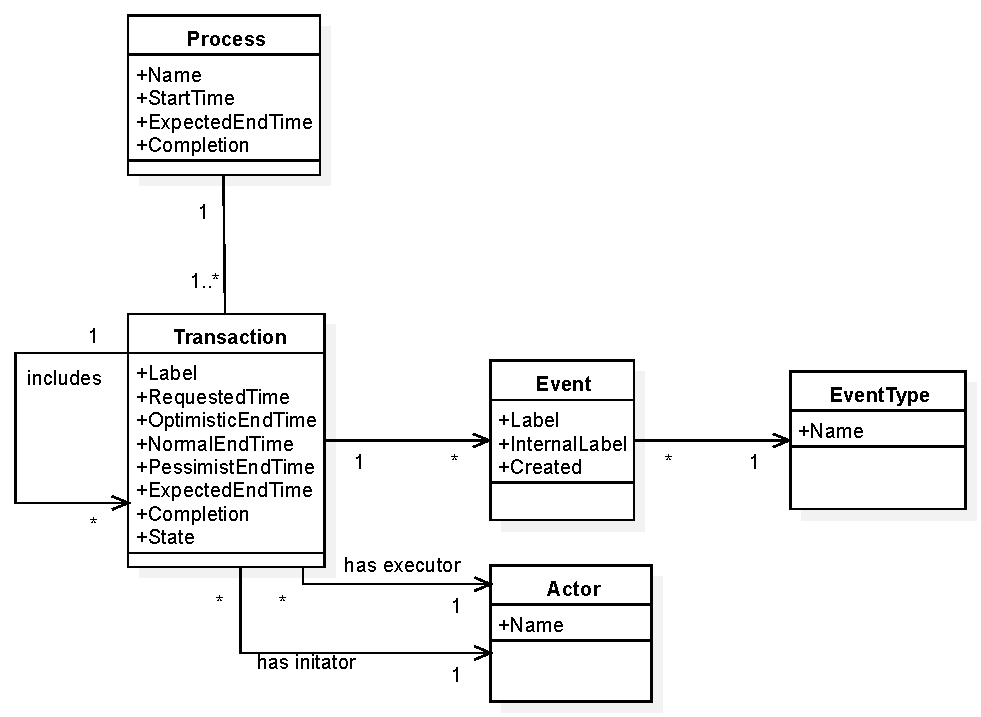
\includegraphics[width=12cm,keepaspectratio]{img/domain-core-model}
        \caption{Domain model \todo{change this image}}
        \label{fig:domain-core-model}
      \end{figure}    
      
      Figure \ref{fig:domain-core-model} shows domain model which describes how collected business data will be transformed for use in mobile application inside overviews and process visualization. 
    
    \section{Overviews}
    
    \section{Process visualization}
    
    \section{Mobile application concept}
	
	\todo{Domain model of collected data. Proposed way of real time visualization. Type of charts. Dashboard. Whole concept of application, e.g dashboard, editor. Functional specification, a.k.a example use cases?? Domain model of collected data.}
% 	\section{Functional specification \todo{Maybe Example use cases}}    
%    \gls{dwma} is mobile-based application that allows managers to create reports over business data. DWMA allows create many types of overviews, such as graphs, that exposing critical information about running business processes. Second critical function is real-time based graph which displays current state of one concrete instance of business process. 
    
% 	This specification  is not complete and focuses only what end-user of \gls{dwma} can do. Spec does not discussed any "deeper" algorithms and used technologies at background.
% Also provided screens and any graphic assets are not final. They only serves as better overview of discussed scenarios, because ``A picture is worth a thousand words".

% 	\todo{Info about RAC - insert whole description of RAC?}. 
    
%     \begin{figure}[h]
%           \centering
%           
\includegraphics{img/TODO-image}
%           \caption{\todo{OCD RAC}}
%       \end{figure}   
    
    
% 	\subsection{Scenario 1 - Janno, one of the CEOs}    
%     Janno is one of the two twins and founders of the \gls{rac} company. He use \gls{dwma} every day mainly for ``top-level" overview of company. He created widget about total amount of request for new car rents at the moment. Also he has a widget which displays number of new requests per day for the last week. Beside this widgets he also created widget where is displayed amount of successfully completed process towards quitted requests grouped by weeks.
    
%     Of course Janno is very wondered about his employees and their productivity. For this purpose, he has a couple more widgets on his dashboard. First is pie chart where every employee from distribution department is displayed with percentages for requests-state acts. Second chart displays number of succeeded requests (request was stated and accepted) at the main office for new rental contracts sorted by from highest to lowest and grouped by employee.
   
%    And one of the important indication of successful company is income, outcome and profit. For this Janno has a widget with simple numbers for each indicators.  
   
    
%     \subsection{\todo{Scenario 2}}   
    
    \section{Analysis}    

   

	\section{The dashboard}
    Purpose of dashboard is provide centralized overview of processes such as average waiting time before process is completed or total amount of requests per day. The appearance of dashboard depends on user. \gls{dwma} provides customizable elements called widgets to achieve desired look for every user individually.

    \subsection{Widgets}  
     Widgets are small independent configurable components for displaying collected data from business processes. Each one has purpose. Notice that widgets are only user-friendly view of query above collected data. For editing widgets there is widget editor. User can simply edit properties of widget such as name, category, tags and of course source of data - the query and second important property is the type of widget. There are following types of widgets:
     
     \textbf{The summary widget} (\cref{fig:widget-summary}) provides, by it's name, chart with summarization of collected data. Concrete type of the chart depends on the user and on the data. Summary widget provides several types of charts:
     
     \begin{enumerate}
    	\item \textit{Pie} chart is used to illustrate numerical proportion.         
        \item  \textit{Bar} chart displays categorical data with numerical value.
        %\item \textit{Line}
    \end{enumerate}
      
      \begin{figure}[ht!]
          \centering
          
\includegraphics[width=6cm,keepaspectratio]{img/TODO-image}
          \caption{Summary widget example}
          \label{fig:widget-summary}
      \end{figure}   
    
   	Second type is \textbf{Time period} (\cref{fig:widget-time-period}). Time period displays data in some interval. Typically it can serve as overview \textit{``Number of requests for Rental payment per day"}.        
      
      \begin{figure}[ht!]
          \centering
          
\includegraphics[width=6cm,keepaspectratio]{img/TODO-image}
          \caption{Time period widget example}
          \label{fig:widget-time-period}
      \end{figure}
    
    Last type is \textbf{Single query} (\cref{fig:widget-single-query}) which allows display simple result from query. Prerequisite for query is that query returns one single record. 
      
      \begin{figure}[ht!]
          \centering
          
\includegraphics[width=6cm,keepaspectratio]{img/TODO-image}
          \caption{Single query example}
           \label{fig:widget-single-query}
      \end{figure}       
    
    \subsection{Query editor}
    
    \todo{Information about query editor}
    
    \begin{figure}[ht!]
          \centering
          
\includegraphics[width=6cm,keepaspectratio]{img/TODO-image}
          \caption{\todo{Query editor}}
      \end{figure}   
    
    \section{The real-time overview of process instance}
    \todo{Introduction about gantt chart. Make conversation about classic OCD / PSD diagrams and their pros and cons for visualizations}
    Provides the real-time overview of one concrete process instance.
On the left side is tree-view (like in folder explorer) of transactions. Each transaction has identifier and name.
On the top is the timeline which displays important events from the process. Above timeline is visualization itself. Each transaction is displayed as progress bar with some visual tweak, which will be discussed later.

	Each transaction can be at one of the following state, which has different visual: 
	\todo{Categories}
    
    \begin{description}
    	\item[Not active transaction] Is displayed as greyed out progress bar. It means that this instance of transaction will be probably started at some future time.

        \item[Active transaction] Progress bar is displayed with green colour to show current progress of instance transaction. 
        
        \item[Completed transaction] Progress bar is fulfilled with green colour. It means that given transaction successfully ended (was accepted).
        
        \item[Stopped transaction]. Progress bar changed colour to red which indicates that transaction failed to complete due to fact that it was quitted or stopped. 
    \end{description}
    
    \subsection{Response and waiting links}
    \todo{Change this}
   Each transaction can have several child-transactions and also many conditional links. These conditions are displayed with arrows pointed to another transaction with the condition.
Conditions are divided into two categories.

If the condition is ``Some state of transaction A has to be done before transaction B can start (be requested)", e.g. transaction A must be stated before transaction B can be requested (\cref{fig:request-start-condition}).

	 \begin{figure}
          \centering
          
\includegraphics[width=6cm,keepaspectratio]{img/TODO-image}
          \caption{\todo{Request-start condition}}
          \label{fig:request-start-condition}
      \end{figure}  

If condition is ``Some state of transaction A has to be done before transaction B can be at another state", e.g transaction A must be at least stated before transaction B can be promised (\cref{fig:state-state-condition}).

	 \begin{figure}
          \centering
          
\includegraphics[width=6cm,keepaspectratio]{img/TODO-image}
          \caption{\todo{State-state condition}}
           \label{fig:state-state-condition}
      \end{figure}  


\chapter{Implementation of concept}

\begin{conclusion}
	%sem napište závěr Vaší práce
\end{conclusion}

\bibliographystyle{csn690}
\bibliography{myref.bib}

\appendix

\printglossaries
% \begin{description}
% 	\item[BPM] \todo{to-do}
%     \item[BPMN] \todo{to-do}
%     \item[BPMS] \todo{to-do}
%     \item[DEMO] \todo{to-do}
% 	\item[GUI] Graphical user interface
% 	\item[XML] Extensible markup language
% \end{description}


\chapter{Content of enclosed CD}

%upravte podle skutecnosti

\begin{figure}
	\dirtree{%
		.1 readme.txt\DTcomment{stručný popis obsahu CD}.
		.1 exe\DTcomment{adresář se spustitelnou formou implementace}.
		.1 src.
		.2 impl\DTcomment{zdrojové kódy implementace}.
		.2 thesis\DTcomment{zdrojová forma práce ve formátu \LaTeX{}}.
		.1 text\DTcomment{text práce}.
		.2 thesis.pdf\DTcomment{text práce ve formátu PDF}.
		.2 thesis.ps\DTcomment{text práce ve formátu PS}.
	}
\end{figure}

\end{document}
